\documentclass[10.5pt]{ctexart}
\usepackage{graphicx}
\usepackage{indentfirst}
\usepackage[a4paper, inner=1.5cm, outer=3cm, top=2cm, bottom=3cm, bindingoffset=1cm]{geometry}
\usepackage{epstopdf}
\usepackage{array}
\usepackage{fontspec}
\usepackage{gensymb}
\usepackage[lofdepth,lotdepth]{subfig}
\setlength{\extrarowheight}{4pt}
\begin{document}
\title{\textbf{\fontsize{15.75pt}{\baselineskip}{电导法测定乙酸乙酯皂化反应速率常数实验报告}}} % 15.75pt is 3 号 in chinese
\author{\fontsize{12pt}{\baselineskip}{数33 赵丰 2013012178 \quad }}
\date{\fontsize{12pt}{\baselineskip}{10 10,2016}}
\maketitle
\section{\textbf{\fontsize{12pt}{\baselineskip}{引言}}}
本次实验用电导法测定乙酸乙酯皂化反应速率常数,反应的化学方程式为:
\begin{equation}
CH_3COOC_2H_5+OH^-\rightleftharpoons CH_3COO^-+C_2H_5OH
\end{equation}
该反应是一个二级反应,若设乙酸乙酯的浓度为c,则反应速率的方程式为:
\begin{equation}
-\frac{d c}{dt}=kc^2
\end{equation}
可以求得c与t的关系为:$\frac{1}{c}-\frac{1}{c_0}=kt$。
若设$G_0,G_t,G_{\infty}$分别为反应起始(刚混合的瞬间)时、反应时间为t时刻以及反应结束时溶液的电导,
则有$G_t=G_0 \frac{c}{c_0}+G_{\infty} \frac{c_0-c}{c_0}$\\
将上两式联立,消去c可得
\begin{equation}
G_t=-ktc_0(G_t-G_{\infty})+G_0
\end{equation}
以$G_t$对$(G_t-G_{\infty})t$作图,可得一直线,直线的斜率为$-kc_0$,从而可求出反应速率常数k。
反应的活化能可根据\textbf{Arrhennius}公式求出
\begin{equation}
\ln(k)=-\frac{E_a}{RT}+\ln(A)
\end{equation}
测出不同温度下的k值,以$\ln(k)$对$\frac{1}{T}$作图可求出反应的活化能$E_a$。
\section{\textbf{\fontsize{12pt}{\baselineskip}{实验操作}}}

\subsection{\textbf{\fontsize{12pt}{\baselineskip}{实验操作步骤及方法要点}}}
\begin{enumerate}
\item 根据助教配得的NaOH溶液的浓度为0.0179mol/L,用容量瓶配制等浓度的乙酸乙酯溶液。
\item 将反应池放入恒温槽中,两边分别加入20mL NaOH和乙酸乙酯,在一端插入测试电极,另一端用洗耳球将溶液压入反应池的对侧,使反应液混合,电导测试仪每1s采集一次数据,反应持续时间大约20分钟。
\item 反应结束后,测定同温度下0.01mol/L的乙酸钠的电导率,作为$G_{\infty}$的近似值。
\item 升高恒温槽的温度,重复(2)、(3)步骤,测出不同温度下电导率随时间变化的关系。
\end{enumerate}
\section{\textbf{\fontsize{12pt}{\baselineskip}{结果与讨论}}}
\subsection{\textbf{\fontsize{12pt}{\baselineskip}{原始实验数据}}}
通过计算得到应量取纯乙酸乙酯液体0.175mL。
实验分别在三个不同的温度下进行,结果如下表所示;
\begin{table}[!ht]
\centering
\caption{实验结果}
\begin{tabular}{ccc}
\hline
温度(\degree C) & 乙酸钠的电导率$(\mu s/cm)$& $k(L/(mol \cdot min))$ \\
\hline
20.1 & 620.33 & 3.78\\
20.55 & 631.5 & 4.01\\
23.4 & 674 & 5.24 \\
\hline
\end{tabular}
\end{table}
三种温度条件下$G_t$对$(G_t-G_{\infty})t$作图均近似为直线,下面只给出T=20.55\degree C时的图形:
\begin{figure}[!ht]
  \centering
  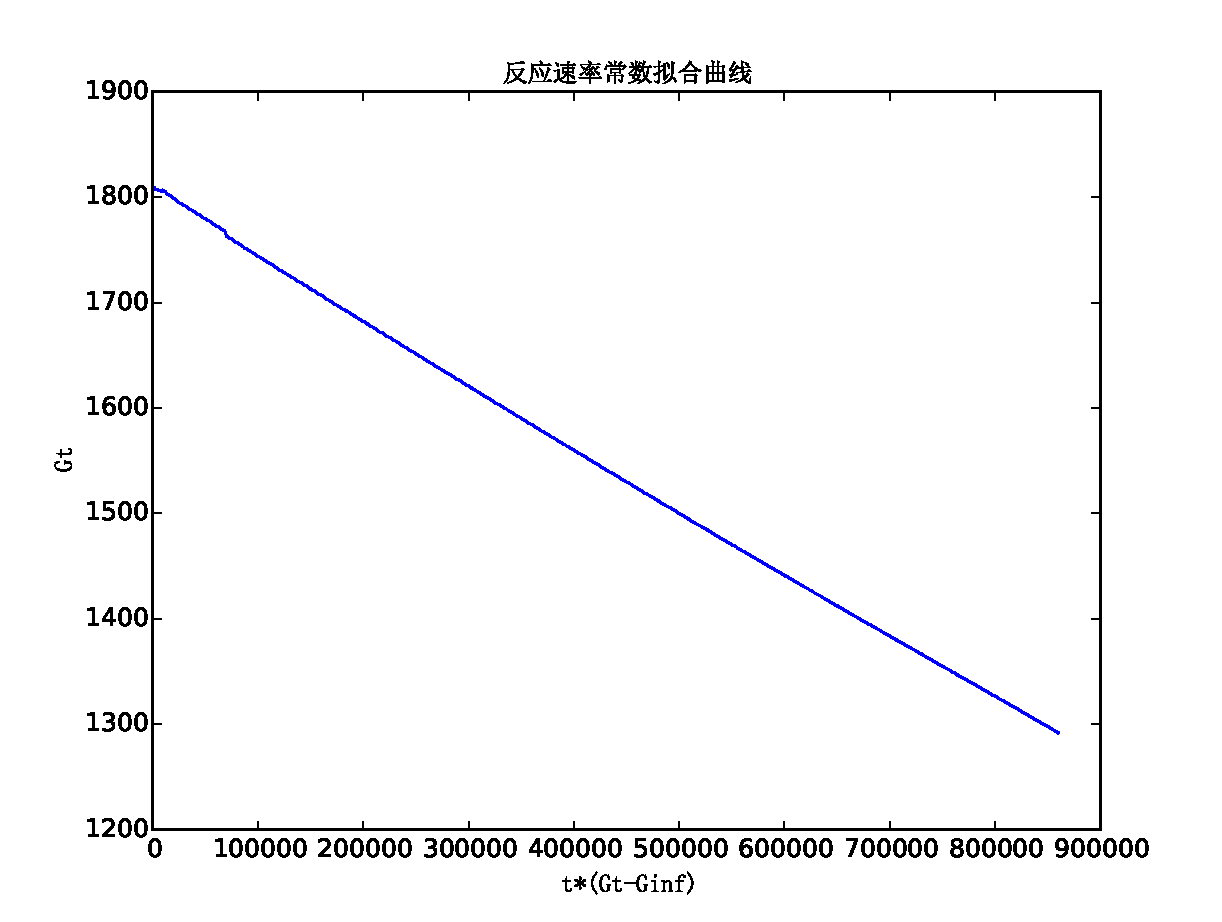
\includegraphics[width=400pt]{figure1.pdf}
\end{figure}

\subsection{\textbf{\fontsize{12pt}{\baselineskip}{计算的数据、结果}}}


由表格中的数据可求得反应的活化能为70.3kJ/mol,文献值这43.1kJ/mol,相差较大。


\subsection{\textbf{\fontsize{12pt}{\baselineskip}{讨论分析}}}
本次实验误差较大,可能的原因有量取乙酸乙酯液体可能有较大偏差,实验后测定0.01mol/L乙酸钠的电导率存在系统误差,应测定0.00875mol/L的乙酸钠的电导率,反应中不恒温,反应后读取温度计示数有较大偏差等。

\section{\textbf{\fontsize{12pt}{\baselineskip}{结论}}}

通过本次实验,我们得出如下结论:
\begin{enumerate}
\item 本次实验使用电导法测浓度,进而推算反应速率常数,但必须精确控制实验条件才能得到较准确的结果。
\end{enumerate}

\section{\textbf{\fontsize{12pt}{\baselineskip}{参考文献}}}
\begin{thebibliography}{}
\bibitem{Bib1}物理化学实验 \quad 化学工业出版社
\end{thebibliography}
\end{document}